
\newcommand{\p}{\textbf{p}}

\chapter{Nonparametric Models}

In this chapter we describe a Bayesian nonparametric approach to inducing the categories in a synchronous context-free grammar.  As discussed in Chapter~\ref{chapter:setup}, we hypothesize that each phrase pair, $\p$, can be clustered on the basis of the contexts it occurs in.  Using this as our starting point, we define a generative model where contexts are generated by the (latent) category type of the phrases they occur in.  In contrast to most prior work using Bayesian models for synchronous grammar induction \citep{blunsom:nips2008,blunsom:acl2009,zhang:2008}, we do not model parallel sentence pairs directly.  Rather, we assume that our corpus is a {\emph collection of contexts}, grouped according to the phrases they occur in, and where each context is conditionally independent of the others, given the type of the category it surrounds.  The models used here are thus variations on the Latent Dirichlet Allocation (LDA) model of \cite{blei:2003}.

In Section~\ref{sec:npmodel} we describe the basic structure of our nonparametric models as well as how inference was carried out.

\section{Model}
\label{sec:npmodel}

This section describes the details of the phrase clustering model.  Each observed phrase (pair), $\p$, is characterized by a finite mixture of categories, $\theta_{\p}$.  The collection of contexts for each phrase, $C_{\p}$, is generated as follows.  A category type $z_i$ is drawn from $\theta_{\p}$, and this generates the observed context, $\textbf{c}_i$, according to a category-specific distribution over contexts types, $\phi_{z_i}$.  Since we do not know the values of $\theta_{\p}$ and $\phi_z$, we place priors on the distributions, to reflect our prior beliefs about the shape these distributions should have and infer their values from the data we can observe.  Specifically, our {\emph a priori} expectation is that both parameters will be relatively peaked, since each phrase, $\p$, should relatively unambiguous belong to particular category, and each category to generate a relatively small number of context strings, $\textbf{c}$. To encode these intuitions, we make use of Pitman-Yor processes \citep{pitman:1997}, which have already been demonstrated to be particularly effective models for language \citep{teh:2006,goldwater:2006}.

Our model assumes a fixed number of categories, $K$. The category type, $z \in \{ 1 , 2 , \ldots , K \}$, is generated from a PYP with a uniform base distribution:
\begin{align*}
z &| \p & \sim \theta_{\p} \\
\theta_{\p} &| a_{\p},b_{\p},K & \sim \textrm{PYP}(a_{\p},b_{\p},\frac{1}{K})
\end{align*}
\noindent As a variation on this, we define a variant of the model with a hierarchical prior on the distribution over categories for a phrase.  We share statistics about category use across phrases, encourage a more peaked distribution of categories:
\begin{align*}
z &| \p & \sim \theta_{\p} \\
\theta_{\p} &| a_{\p},b_{\p} & \sim \textrm{PYP}(a_{\p},b_{\p},\theta_0) \\
\theta_0 &| a_0,b_0,K & \sim \textrm{PYP}(a_0,b_0,\frac{1}{K})
\end{align*}

\noindent Now that we have described how category labels are generated, we describe how contexts are generated from the category.  We again model this process using a PYP. Not only does this model tend to favor solutions where contexts used repeatedly are clustered, but it provides a natural way to do smoothing.  Since many contexts may be only infrequently observed in the training data, proper smoothing is crucial.  Specifically, we can smooth specific contexts by backing off to less specific contexts (e.g., composed of fewer words or word classes).

The most basic version of our model uses a uniform base distribution over contexts. This model was most useful when generating contexts consisting of a single word or word class (i.e., $\textbf{c}=c_{-1}c_1$) in either the source or target language on either side.

\begin{align*}
c_{-1}c_1 |& z & \sim \phi_z \\
\phi_z |& a_z,b_z & \sim \textrm{PYP}(a_z,b_z,\frac{1}{|V|^2})
\end{align*}

\noindent When larger contexts were used, the space of these contexts becomes very sparse, so another variant of our model uses a non-uniform base distribution to back off to the probability of generating a smaller context (i.e., $c_{-1}c_1$) as above and then generating the outer context

\begin{align*}
c_{-2}c_{-1}c_1c_2 |& z & \sim \phi_z \\
\phi_z |& a_z,b_z & \sim \textrm{PYP}(a_z,b_z,P_1(\cdot|z)) \\
&P_1(c_{-2}c_{-1}c_1c_2|z)& = \phi^{\textrm{\emph{inner}}}_z(c_{-1}c_1|z) \times \frac{1}{|V|^2} \\
c_{-1}c_1 |& z & \sim \phi^{\textrm{\emph{inner}}}_z \\
\phi^{\textrm{\emph{inner}}}_z |& a^{\textrm{\emph{inner}}}_z,b^{\textrm{\emph{inner}}}_z & \sim \textrm{PYP}(a^{\textrm{\emph{inner}}}_z,b^{\textrm{\emph{inner}}}_z,\frac{1}{|V|^2})
\end{align*}

\noindent Figure~\ref{fig:np_plate} shows a plate diagram for the two parts of the model that were just described.

\begin{figure}
\begin{center}
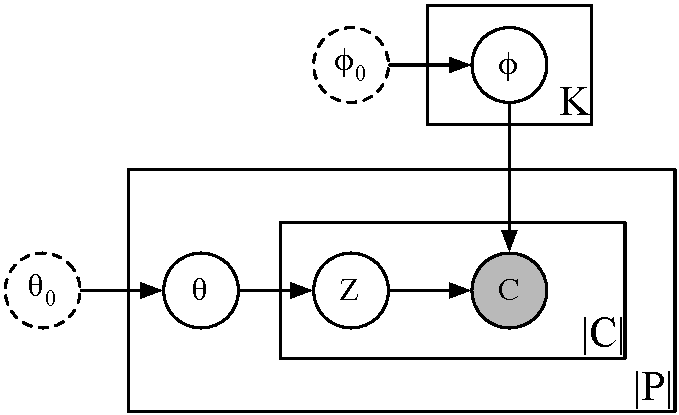
\includegraphics[scale=0.75]{pyp_clustering/np_plate.pdf}
\vspace{-0.3cm}
\end{center}
\caption{Plate diagram for the nonparametric clustering model (hyperparameters omitted).  Dashed circles indicate variables that may not be present in every model.}
\label{fig:np_plate}
\end{figure}

\paragraph{Hyperparameter priors.} The hyperparameters of the PYPs in our models are treated as random variables whose values are inferred from the data and the priors used to characterize the values we expect them to take on.  Since we have only a poor prior understanding about what their appropriate values should be, we use vague priors: discount parameters, $a_{(\cdot)}$, are drawn from a uniform Beta distribution ($a_{(\cdot)} \sim \textrm{Beta}(1,1)$) and concentration parameters, $b_{(\cdot)}$, are drawn from a Gamma distribution ($b_{(\cdot)} \sim \textrm{Gamma}(1,1)$).

\section{Inference}

Inference in the nonparametric clustering models was performed using Gibbs sampling \citep{geman:1984}, with the continuous parameters ($\theta_{\p}$, $\phi_z$, etc.) integrated out \citep{blunsom:2009}.  For the experiments reported below, we sampled for 1,000 iterations.  The initial state of the sampler was created by assigning every context in a phrase entirely to a random category. Values for the PYP hyperparameters were resampled after every 10 samples of the Gibbs sampler using the range doubling slice sampling technique \citep{neal:2000,johnson:2009}. Figure~\ref{fig:llh} shows the log-likelihood of the model measured after every 10 samples on an example run of the Urdu-English data with two different numbers of categories.

The final sample drawn from the model was used to estimate $p(z|\textbf{c},\p)$, and each phrase occurrence was labelled with the $z$ that maximized this probability.

\begin{figure}
\begin{center}
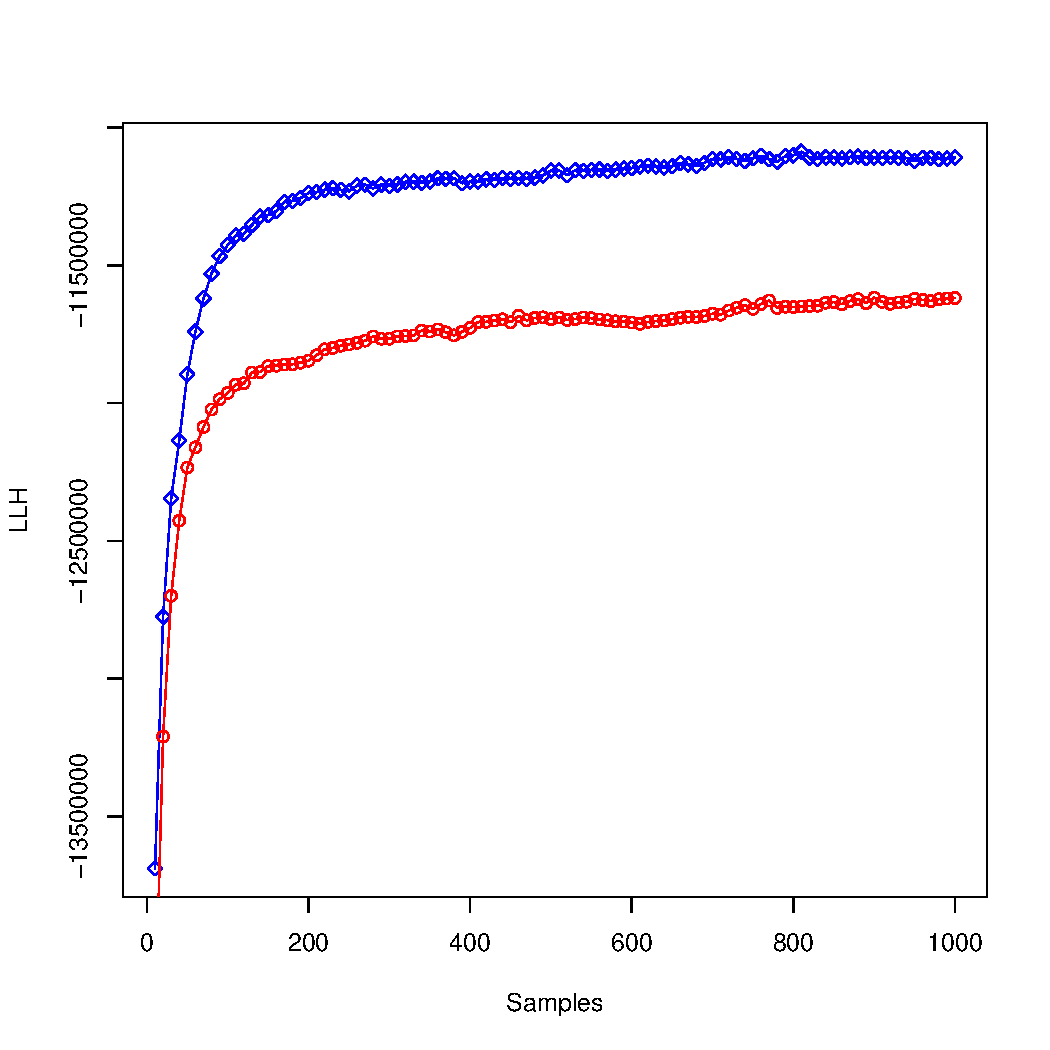
\includegraphics[scale=0.5]{pyp_clustering/llh.pdf}
\vspace{-0.7cm}
\end{center}
\caption{Log-likelihood versus number of samples with 10 categories (red circles) and 25 categories (blue diamonds) on the Urdu data, 1 target word on either side, hierarchical $\theta_0$, uniform $\phi_0$.}
\label{fig:llh}
\end{figure}

\section{Experiments}

This section reports a number of experiments carried out to test the quality of the grammars learned using our nonparametric cluster models.  We evaluate them primarily in terms of their performance on translation tasks.  Translation quality evaluation is reported using case-insensitive \textsc{bleu} \citep{bleu} with the number of references used depending on the experimental condition (refer to details in the discussion of the corpora used below).

\subsection{Corpora}

The experiments reported in this section were carried out primarily on a small Chinese-English corpus from the travel and tourism domain \citep{btec} and a more general-domain Urdu-English corpus, made available by the US National Institute of Standards and Technology (NIST) for the Open MT Evaluation.\footnote{http://www.itl.nist.gov/iad/mig/tests/mt/} Table~\ref{tab:corpbtecur} provides statistics about the training and test data used in the experiments reported in this section.  Additionally, this table gives the number of references used to compute the \textsc{bleu} score for a translated document.

\begin{table}[h]
\caption{Training corpus statistics for BTEC Chinese-English and the NIST Urdu-English data sets.}
\begin{center}
\begin{tabular}{l|r|r}
& BTEC & Urdu \\
\hline
Sentences & 44,016 & 51,214 \\
English types & 9,555 & 31,492 \\
English tokens & 364,297 & 968,013 \\
Foreign types & 13,664 & 33,757 \\
Foreign tokens & 333,438 & 1,052,260 \\
\hline
Dev. sentences & 1,006 & 882 \\
Test sentences & 506 & 883 \\
Num. references & 16 & 4
\end{tabular}
\end{center}
\label{tab:corpbtecur}
\end{table}%

\subsection{Translation system features}

In addition to the language model and word penalty, we made use of the following features to score each rule $\textrm{Y} \rightarrow \langle \textbf{f},\textbf{e} \rangle$ used in a derivation.  Some features are meaningful only in the context of multi-category grammars.

\begin{enumerate}
\item The lexical translation log probability of the words in both phrases, $\log \textrm{{\emph lex}}(\textbf{e}|\textbf{f})$, as defined in \cite{Koehn2003}.
\item The inverse lexical translation log probability, $\log \textrm{{\emph lex}}(\textbf{f}|\textbf{e})$.
\item The log frequency of occurrence of the LHS category, $\log f(\textrm{Y})$. This feature always has a value of 0 in the single category (baseline) system.
\item The relative frequency of \textbf{e} given \textbf{f}, collapsing all non-terminals into the symbol X, $f_{\textbf{X}}(\textbf{e}|\textbf{f})$. This is equivalent to the relative frequency of the rule in the 1-category `Hiero' grammar.
\item The inverse relative frequency, $f_{\textbf{X}}(\textbf{f}|\textbf{e})$.
\item The relative frequency of $\langle \textbf{f}, \textbf{e} \rangle$ given Y, $f(\textbf{f}, \textbf{e} | \textrm{Y})$.
\item The log rule count, $\log C(\textrm{Y} \rightarrow \langle \textbf{f},\textbf{e} \rangle)$.
\item A feature with value 1 (creates a count of the number of rules in the derivation).
\end{enumerate}

\noindent The above feature weights were tuned using the minimum error rate training algorithm (\textsc{mert}), to optimize the 1-best \textsc{bleu} on a held-out development set.

\subsection{Baseline and supervised benchmark systems}

We provide a number of baselines to compare our unsupervised syntax systems against.  The most important is a single-category system constructed using the procedure described by \cite{chiang:2007} The single-category baseline represents the current state-of-the-art for systems that do not utilize supervised syntax or syntax proxies (like POS tags or syntactic chunks).  The random category baselines are provided to give an indication of how a poorly induced syntactic system (for a given $K$) would perform.

Additionally, we also provide two benchmark systems that use a more sensible set of nonterminal categories.  The first uses supervised English (target) language parse trees to annotate the phrases in the grammar as proposed by \cite{samt}.  The second (labeled Target POS-only) uses the target language part-of-speech tag for all rules that generate only a single terminal symbol in the target language, and the symbol X otherwise.

\begin{table}
\caption{Baseline systems}
\begin{center}
\begin{tabular}{r|c|c}
& BTEC & Urdu \\
\hline
Single category \citep{chiang:2007} & 57.0 & 21.1 \\
\hline
Random ($K=10$) & 56.0 & 19.8 \\
Random ($K=25$) & 55.4 & 19.7 \\
Random ($K=50$) &  55.3 & 19.6 \\
\hline
Supervised \citep{samt} & 57.8 & 24.5 \\
Target POS-only ({\emph supervised}) & 56.2 & 22.2 \\
\end{tabular}
\end{center}
\label{tab:npbaselines}
\end{table}%

\subsection{Number of categories}

The number of categories, $K$, is a free parameter in our nonparametric clustering model.  In this section, we report results exploring the effect of $K$ on translation quality on the BTEC and Urdu translation tasks.

Preliminary experiments indicated that single word (to the left and right) target language contexts learned with with a uniform $\phi_0$ and a hierarchical $\theta_0$ produced useful clusters for translation, so we used this as the definition of the context for this experiment. Table~\ref{tab:npvaryk} summarizes the affect of varying $K$ using a single word of target language context, using a uniform $\phi_0$ and a hierarchical $\theta_0$. 

\begin{table}[h]
\caption{Effect of varying $K$, single word left and right target language context, uniform $\phi_0$, hierarchical $\theta_0$.}
\begin{center}
\begin{tabular}{r|c|c}
& BTEC & Urdu \\
\hline
Single category (baseline) & 57.0 & 21.1 \\
\hline
$K=10$ & 56.4 & 21.2 \\
$K=25$ & \textbf{57.5} & \textbf{22.0} \\
$K=50$ & 56.2 & 21.4 \\
\end{tabular}
\end{center}
\label{tab:npvaryk}
\end{table}%


\subsection{Context types}

Because the margin of improvement from the 1-category baseline to the supervised condition is much more substantial in the Urdu-English condition than in the BTEC condition, the experiments in this section were carried out only on Urdu.


\begin{table}[h]
\caption{Effect of varying the context definition and/or smoothing, $K=25$, hierarchical $\theta_0$; best results in bold. Baseline and benchmark systems also included for reference.}
\begin{center}
\begin{tabular}{r|c|c|c|c}
Context Type & $|\textbf{c}|/2$ & $\phi_0$ & \textsc{bleu} & $H(S|Z)$ \\
\hline
Baseline ($K=1$) & -- & -- & 20.9 &  4.49 \\
\hline
Source word & 1 & uniform & 21.7 & 3.25 \\
Source word class & 1 & uniform & 20.4 & 3.03 \\
Target word & 1 & uniform & 22.0 & 2.86 \\
Target word class & 1 & uniform & \textbf{22.3} & \textbf{2.27} \\
Source word & 2 & 1-word backoff & 21.3 & 3.41 \\
Source word class & 2 & 1-class backoff & & 4.20 \\
Target word & 2 & 1-word backoff & 20.8 & 3.16 \\
Target word class & 2 & 1-class backoff & 20.1 & 4.06 \\
\hline
Supervised \citep{samt} & -- & -- & 24.6 & 0 \\
Target POS-only ({\emph supervised}) & 1 & uniform & 22.2 & 1.85 \\
\end{tabular}
\end{center}
\label{tab:npbaselines}
\end{table}%

\subsection{Correlating the intrinsic metric}

\begin{figure}
\begin{center}
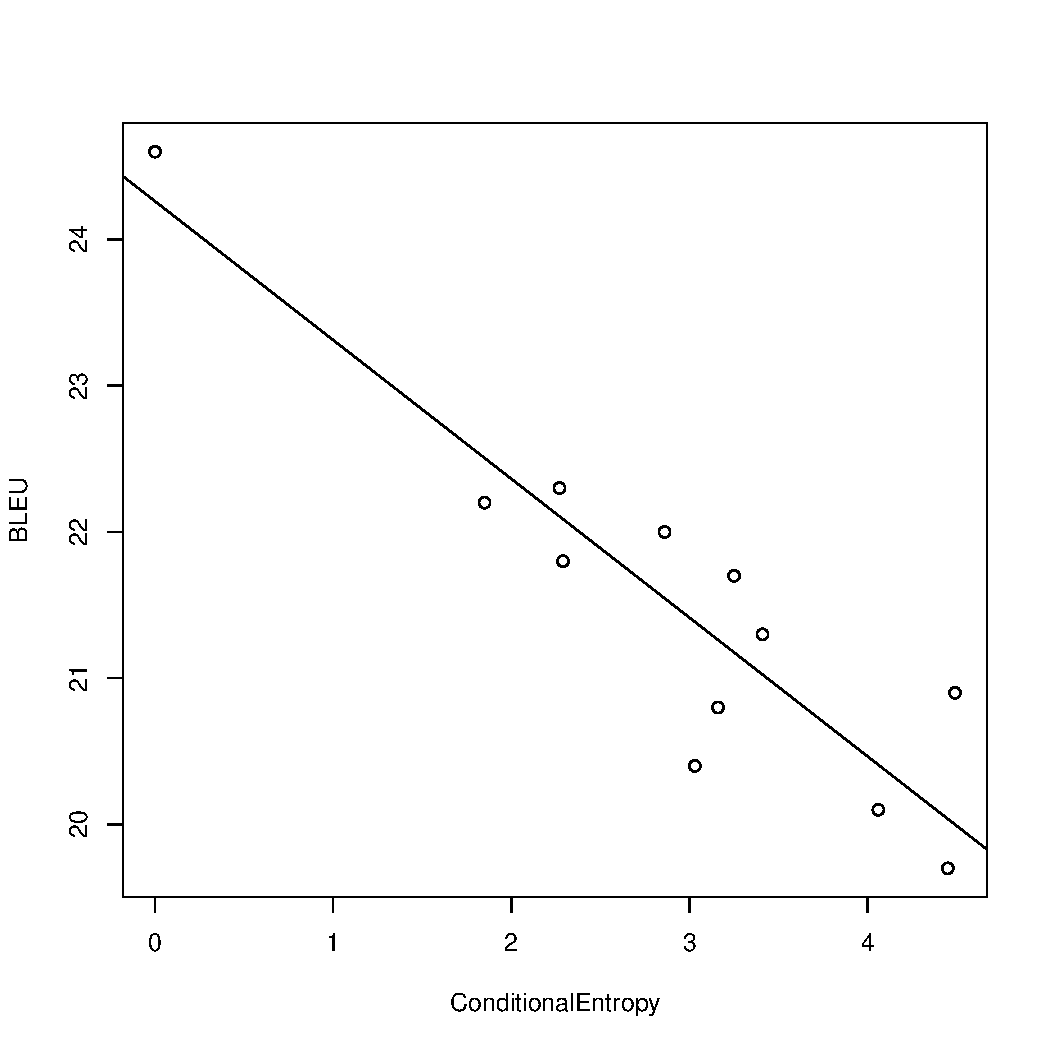
\includegraphics[scale=0.5]{pyp_clustering/correl.pdf}
\vspace{-0.3cm}
\end{center}
\caption{The intrinsic conditional entropy metric $H(S|Z)$ correlates approximately linearly with \textsc{bleu}.}
\label{fig:intr_correl}
\end{figure}


\section{Discussion}

\subsection{Qualitative analysis of an example grammar}

Tables~\ref{tab:npexample1} and \ref{tab:npexample2} show a fragment of a 25-category Urdu-English grammar learned using the nonparametric phrase clustering.  Rules were selected that maximized the relative frequency $p(\textrm{RHS}|\textrm{LHS})$, filtering out the top 25 (to minimize the appearance of frequent words), and showing only rules consisting of terminal symbols in their right hand side (for clarity). The frequency of each rule type in a grammar filtered for the development set is also given.

\begin{table}[h]
\caption{Fragment (part 1/2) of 25 category Urdu-English grammar, hierarchical $\theta_0$, uniform $\phi_0$, 1 word context on either side in the target language. Counts indicate the number of distinct rules that rewrite each category type. For clarity, only rules containing only terminal symbols in their RHS are shown.}
\begin{center}
\begin{tabular}{|c|l|c|l|}
\hline
22,386 & $ \textrm{X}^{0} \rightarrow \langle \textrm{EdAlt},\textrm{{\emph court}} \rangle $ &27,604 & $ \textrm{X}^{8} \rightarrow \langle \textrm{tHt},\textrm{{\emph under}} \rangle $ \\
 & $ \textrm{X}^{0} \rightarrow \langle \textrm{bcwN},\textrm{{\emph children}} \rangle $ & & $ \textrm{X}^{8} \rightarrow \langle \textrm{myN},\textrm{{\emph into}} \rangle $ \\
 & $ \textrm{X}^{0} \rightarrow \langle \textrm{lwg},\textrm{{\emph people}} \rangle $ & & $ \textrm{X}^{8} \rightarrow \langle \textrm{yA},\textrm{{\emph or}} \rangle $ \\
 & $ \textrm{X}^{0} \rightarrow \langle \textrm{bcY},\textrm{{\emph children}} \rangle $ & & $ \textrm{X}^{8} \rightarrow \langle \textrm{ky},\textrm{{\emph for}} \rangle $ \\
 & $ \textrm{X}^{0} \rightarrow \langle \textrm{ArkAn},\textrm{{\emph members}} \rangle $ & & $ \textrm{X}^{8} \rightarrow \langle \textrm{kY},\textrm{{\emph for}} \rangle $ \\
\hline
26,834 & $ \textrm{X}^{1} \rightarrow \langle \textrm{Drwrt},\textrm{{\emph need}} \rangle $ &40,283 & $ \textrm{X}^{9} \rightarrow \langle \textrm{3},\textrm{{\emph 3}} \rangle $ \\
 & $ \textrm{X}^{1} \rightarrow \langle \textrm{SHAfywN},\textrm{{\emph journalists}} \rangle $ & & $ \textrm{X}^{9} \rightarrow \langle \textrm{Hsyn},\textrm{{\emph hussein}} \rangle $ \\
 & $ \textrm{X}^{1} \rightarrow \langle \textrm{bAt},\textrm{{\emph speak}} \rangle $ & & $ \textrm{X}^{9} \rightarrow \langle \textrm{fArwq},\textrm{{\emph farooq}} \rangle $ \\
 & $ \textrm{X}^{1} \rightarrow \langle \textrm{HSh},\textrm{{\emph participate}} \rangle $ & & $ \textrm{X}^{9} \rightarrow \langle \textrm{AqbAl},\textrm{{\emph iqbal}} \rangle $ \\
 & $ \textrm{X}^{1} \rightarrow \langle \textrm{Apyl},\textrm{{\emph appeal}} \rangle $ & & $ \textrm{X}^{9} \rightarrow \langle \textrm{bn},\textrm{{\emph bin}} \rangle $ \\
\hline
61,592 & $ \textrm{X}^{2} \rightarrow \langle \textrm{kr},\textrm{{\emph the}} \rangle $ &182,196 & $ \textrm{X}^{10} \rightarrow \langle \textrm{yhAN},\textrm{{\emph here}} \rangle $ \\
 & $ \textrm{X}^{2} \rightarrow \langle \textrm{hmArY},\textrm{{\emph our}} \rangle $ & & $ \textrm{X}^{10} \rightarrow \langle \textrm{AjlAs myN},\textrm{{\emph in the meeting}} \rangle $ \\
 & $ \textrm{X}^{2} \rightarrow \langle \textrm{ErAqy},\textrm{{\emph iraqi}} \rangle $ & & $ \textrm{X}^{10} \rightarrow \langle \textrm{AysA},\textrm{{\emph so}} \rangle $ \\
 & $ \textrm{X}^{2} \rightarrow \langle \textrm{dwsrY},\textrm{{\emph other}} \rangle $ & & $ \textrm{X}^{10} \rightarrow \langle \textrm{ElAj},\textrm{{\emph treatment}} \rangle $ \\
 & $ \textrm{X}^{2} \rightarrow \langle \textrm{pr},\textrm{{\emph the}} \rangle $ & & $ \textrm{X}^{10} \rightarrow \langle \textrm{b@hrt},\textrm{{\emph india}} \rangle $ \\
\hline
98,970 & $ \textrm{X}^{3} \rightarrow \langle \textrm{zndgy},\textrm{{\emph life}} \rangle $ &7,648 & $ \textrm{X}^{11} \rightarrow \langle \textrm{sktA},\textrm{{\emph could}} \rangle $ \\
 & $ \textrm{X}^{3} \rightarrow \langle \textrm{brTAnyh},\textrm{{\emph britain}} \rangle $ & & $ \textrm{X}^{11} \rightarrow \langle \textrm{skyN},\textrm{{\emph can}} \rangle $ \\
 & $ \textrm{X}^{3} \rightarrow \langle \textrm{sEwdy Erb},\textrm{{\emph saudi arabia}} \rangle $ & & $ \textrm{X}^{11} \rightarrow \langle \textrm{tRym},\textrm{{\emph team}} \rangle $ \\
 & $ \textrm{X}^{3} \rightarrow \langle \textrm{AslAm},\textrm{{\emph islam}} \rangle $ & & $ \textrm{X}^{11} \rightarrow \langle \textrm{kAm},\textrm{{\emph work}} \rangle $ \\
 & $ \textrm{X}^{3} \rightarrow \langle \textrm{cyn},\textrm{{\emph china}} \rangle $ & & $ \textrm{X}^{11} \rightarrow \langle \textrm{\$mAly},\textrm{{\emph north}} \rangle $ \\
\hline
66,916 & $ \textrm{X}^{4} \rightarrow \langle \textrm{AnSAf},\textrm{{\emph justice}} \rangle $ &58,760 & $ \textrm{X}^{12} \rightarrow \langle \textrm{tryn},\textrm{{\emph most}} \rangle $ \\
 & $ \textrm{X}^{4} \rightarrow \langle \textrm{bynk},\textrm{{\emph bank}} \rangle $ & & $ \textrm{X}^{12} \rightarrow \langle \textrm{wAlA},\textrm{{\emph man}} \rangle $ \\
 & $ \textrm{X}^{4} \rightarrow \langle \textrm{nZAm},\textrm{{\emph system}} \rangle $ & & $ \textrm{X}^{12} \rightarrow \langle \textrm{ksy},\textrm{{\emph one}} \rangle $ \\
 & $ \textrm{X}^{4} \rightarrow \langle \textrm{rws},\textrm{{\emph russia}} \rangle $ & & $ \textrm{X}^{12} \rightarrow \langle \textrm{sb},\textrm{{\emph most}} \rangle $ \\
 & $ \textrm{X}^{4} \rightarrow \langle \textrm{srHd},\textrm{{\emph nwfp}} \rangle $ & & $ \textrm{X}^{12} \rightarrow \langle \textrm{bED},\textrm{{\emph some}} \rangle $ \\
\hline
29,526 & $ \textrm{X}^{5} \rightarrow \langle \textrm{qbwl},\textrm{{\emph accept}} \rangle $ &80,567 & $ \textrm{X}^{13} \rightarrow \langle \textrm{Amrykh kY},\textrm{{\emph the united}} \rangle $ \\
 & $ \textrm{X}^{5} \rightarrow \langle \textrm{cAhtY},\textrm{{\emph want}} \rangle $ & & $ \textrm{X}^{13} \rightarrow \langle \textrm{"},\textrm{{\emph "}} \rangle $ \\
 & $ \textrm{X}^{5} \rightarrow \langle \textrm{jAntY},\textrm{{\emph know}} \rangle $ & & $ \textrm{X}^{13} \rightarrow \langle \textrm{kl},\textrm{{\emph tomorrow}} \rangle $ \\
 & $ \textrm{X}^{5} \rightarrow \langle \textrm{dY},\textrm{{\emph give}} \rangle $ & & $ \textrm{X}^{13} \rightarrow \langle \textrm{mjls},\textrm{{\emph majlis}} \rangle $ \\
 & $ \textrm{X}^{5} \rightarrow \langle \textrm{bcAnY},\textrm{{\emph save}} \rangle $ & & $ \textrm{X}^{13} \rightarrow \langle \textrm{Awr pAkstAn},\textrm{{\emph and pakistan}} \rangle $ \\
\hline
12,625 & $ \textrm{X}^{6} \rightarrow \langle \textrm{dAxlh},\textrm{{\emph interior}} \rangle $ &111,291 & $ \textrm{X}^{14} \rightarrow \langle \textrm{pAkstAn myN},\textrm{{\emph in pakistan}} \rangle $ \\
 & $ \textrm{X}^{6} \rightarrow \langle \textrm{myjr},\textrm{{\emph major}} \rangle $ & & $ \textrm{X}^{14} \rightarrow \langle \textrm{xw\$},\textrm{{\emph happy}} \rangle $ \\
 & $ \textrm{X}^{6} \rightarrow \langle \textrm{Erb},\textrm{{\emph arab}} \rangle $ & & $ \textrm{X}^{14} \rightarrow \langle \textrm{\$rkt},\textrm{{\emph participated}} \rangle $ \\
 & $ \textrm{X}^{6} \rightarrow \langle \textrm{nY btAyA},\textrm{{\emph told}} \rangle $ & & $ \textrm{X}^{14} \rightarrow \langle \textrm{kAmyAb},\textrm{{\emph succeeded}} \rangle $ \\
 & $ \textrm{X}^{6} \rightarrow \langle \textrm{dAxlh},\textrm{{\emph home}} \rangle $ & & $ \textrm{X}^{14} \rightarrow \langle \textrm{nArAD},\textrm{{\emph angry}} \rangle $ \\
\hline
53,541 & $ \textrm{X}^{7} \rightarrow \langle \textrm{bcY},\textrm{{\emph child}} \rangle $ &8,547 & $ \textrm{X}^{15} \rightarrow \langle \textrm{hy},\textrm{{\emph is}} \rangle $ \\
 & $ \textrm{X}^{7} \rightarrow \langle \textrm{Hq},\textrm{{\emph right}} \rangle $ & & $ \textrm{X}^{15} \rightarrow \langle \textrm{hw gy},\textrm{{\emph will be}} \rangle $ \\
 & $ \textrm{X}^{7} \rightarrow \langle \textrm{\$hr},\textrm{{\emph city}} \rangle $ & & $ \textrm{X}^{15} \rightarrow \langle \textrm{hw},\textrm{{\emph have}} \rangle $ \\
 & $ \textrm{X}^{7} \rightarrow \langle \textrm{SwrtHAl},\textrm{{\emph situation}} \rangle $ & & $ \textrm{X}^{15} \rightarrow \langle \textrm{rhy hY},\textrm{{\emph is}} \rangle $ \\
 & $ \textrm{X}^{7} \rightarrow \langle \textrm{jng},\textrm{{\emph war}} \rangle $ & & $ \textrm{X}^{15} \rightarrow \langle \textrm{kA},\textrm{{\emph 's}} \rangle $ \\
\hline
\end{tabular}
\end{center}
\label{tab:npexample1}
\end{table}%

\begin{table}[h]
\caption{Fragment (part 2/2) of 25 category Urdu-English grammar.}
\begin{center}
\begin{tabular}{|c|l|c|l|}
\hline
40,738 & $ \textrm{X}^{16} \rightarrow \langle \textrm{gyA},\textrm{{\emph .}} \rangle $ &68,633 & $ \textrm{X}^{20} \rightarrow \langle \textrm{m\$yn},\textrm{{\emph machine}} \rangle $ \\
 & $ \textrm{X}^{16} \rightarrow \langle \textrm{lyA},\textrm{{\emph .}} \rangle $ & & $ \textrm{X}^{20} \rightarrow \langle \textrm{myN mwjwd},\textrm{{\emph present in}} \rangle $ \\
 & $ \textrm{X}^{16} \rightarrow \langle \textrm{dy},\textrm{{\emph .}} \rangle $ & & $ \textrm{X}^{20} \rightarrow \langle \textrm{AZhAr},\textrm{{\emph expressing}} \rangle $ \\
 & $ \textrm{X}^{16} \rightarrow \langle \textrm{hy},\textrm{{\emph .}} \rangle $ & & $ \textrm{X}^{20} \rightarrow \langle \textrm{jyt},\textrm{{\emph winning}} \rangle $ \\
 & $ \textrm{X}^{16} \rightarrow \langle \textrm{, pAkstAn},\textrm{{\emph , pakistan}} \rangle $ & & $ \textrm{X}^{20} \rightarrow \langle \textrm{nhyN},\textrm{{\emph not}} \rangle $ \\
\hline
16,270 & $ \textrm{X}^{17} \rightarrow \langle \textrm{pr},\textrm{{\emph to}} \rangle $ &40,443 & $ \textrm{X}^{21} \rightarrow \langle \textrm{AnkAr},\textrm{{\emph refused}} \rangle $ \\
 & $ \textrm{X}^{17} \rightarrow \langle \textrm{sy},\textrm{{\emph to}} \rangle $ & & $ \textrm{X}^{21} \rightarrow \langle \textrm{khnA},\textrm{{\emph according}} \rangle $ \\
 & $ \textrm{X}^{17} \rightarrow \langle \textrm{AnhwN nY},\textrm{{\emph he further}} \rangle $ & & $ \textrm{X}^{21} \rightarrow \langle \textrm{mlAqAt},\textrm{{\emph met}} \rangle $ \\
 & $ \textrm{X}^{17} \rightarrow \langle \textrm{mstRr jstRs},\textrm{{\emph mr. justice}} \rangle $ & & $ \textrm{X}^{21} \rightarrow \langle \textrm{nY},\textrm{{\emph gave}} \rangle $ \\
 & $ \textrm{X}^{17} \rightarrow \langle \textrm{nY},\textrm{{\emph he}} \rangle $ & & $ \textrm{X}^{21} \rightarrow \langle \textrm{sykwrtRy},\textrm{{\emph security}} \rangle $ \\
\hline
90,448 & $ \textrm{X}^{18} \rightarrow \langle \textrm{jhAN},\textrm{{\emph where}} \rangle $ &573,610 & $ \textrm{X}^{22} \rightarrow \langle \textrm{w},\textrm{{\emph and}} \rangle $ \\
 & $ \textrm{X}^{18} \rightarrow \langle \textrm{kh},\textrm{{\emph "}} \rangle $ & & $ \textrm{X}^{22} \rightarrow \langle \textrm{)},\textrm{{\emph )}} \rangle $ \\
 & $ \textrm{X}^{18} \rightarrow \langle \textrm{tAkh},\textrm{{\emph so}} \rangle $ & & $ \textrm{X}^{22} \rightarrow \langle \textrm{nY},\textrm{{\emph ,}} \rangle $ \\
 & $ \textrm{X}^{18} \rightarrow \langle \textrm{dryN AvnA'},\textrm{{\emph meanwhile}} \rangle $ & & $ \textrm{X}^{22} \rightarrow \langle \textrm{bEd},\textrm{{\emph after}} \rangle $ \\
 & $ \textrm{X}^{18} \rightarrow \langle \textrm{smyt},\textrm{{\emph including}} \rangle $ & & $ \textrm{X}^{22} \rightarrow \langle \textrm{(},\textrm{{\emph (}} \rangle $ \\
\hline
64,006 & $ \textrm{X}^{19} \rightarrow \langle \textrm{pwlys},\textrm{{\emph police}} \rangle $ &80,463 & $ \textrm{X}^{23} \rightarrow \langle \textrm{ElAqY},\textrm{{\emph area}} \rangle $ \\
 & $ \textrm{X}^{19} \rightarrow \langle \textrm{whAN},\textrm{{\emph there}} \rangle $ & & $ \textrm{X}^{23} \rightarrow \langle \textrm{bynk},\textrm{{\emph bank}} \rangle $ \\
 & $ \textrm{X}^{19} \rightarrow \langle \textrm{lwg},\textrm{{\emph people}} \rangle $ & & $ \textrm{X}^{23} \rightarrow \langle \textrm{brAdry},\textrm{{\emph community}} \rangle $ \\
 & $ \textrm{X}^{19} \rightarrow \langle \textrm{As},\textrm{{\emph there}} \rangle $ & & $ \textrm{X}^{23} \rightarrow \langle \textrm{Erb},\textrm{{\emph arabia}} \rangle $ \\
 & $ \textrm{X}^{19} \rightarrow \langle \textrm{myrA},\textrm{{\emph i}} \rangle $ & & $ \textrm{X}^{23} \rightarrow \langle \textrm{mslm lyg},\textrm{{\emph muslim league}} \rangle $ \\
\hline
 22,525 & $ \textrm{X}^{24} \rightarrow \langle \textrm{Drwry},\textrm{{\emph necessary}} \rangle $ &&\\
 & $ \textrm{X}^{24} \rightarrow \langle \textrm{m\$kl},\textrm{{\emph difficult}} \rangle $ &&\\
 & $ \textrm{X}^{24} \rightarrow \langle \textrm{mkml},\textrm{{\emph completed}} \rangle $ && \\
 & $ \textrm{X}^{24} \rightarrow \langle \textrm{jA},\textrm{{\emph being}} \rangle $ &&\\
 & $ \textrm{X}^{24} \rightarrow \langle \textrm{AjAzt},\textrm{{\emph allowed}} \rangle $&& \\
\hline

\end{tabular}
\end{center}
\label{tab:npexample2}
\end{table}%


